\documentclass[tikz,border=1mm]{standalone}
\usepackage[T1]{fontenc}
\usepackage[dvipsnames]{xcolor}
\usepackage{pgfplots}

\pgfplotsset{compat=1.18}

\begin{document}

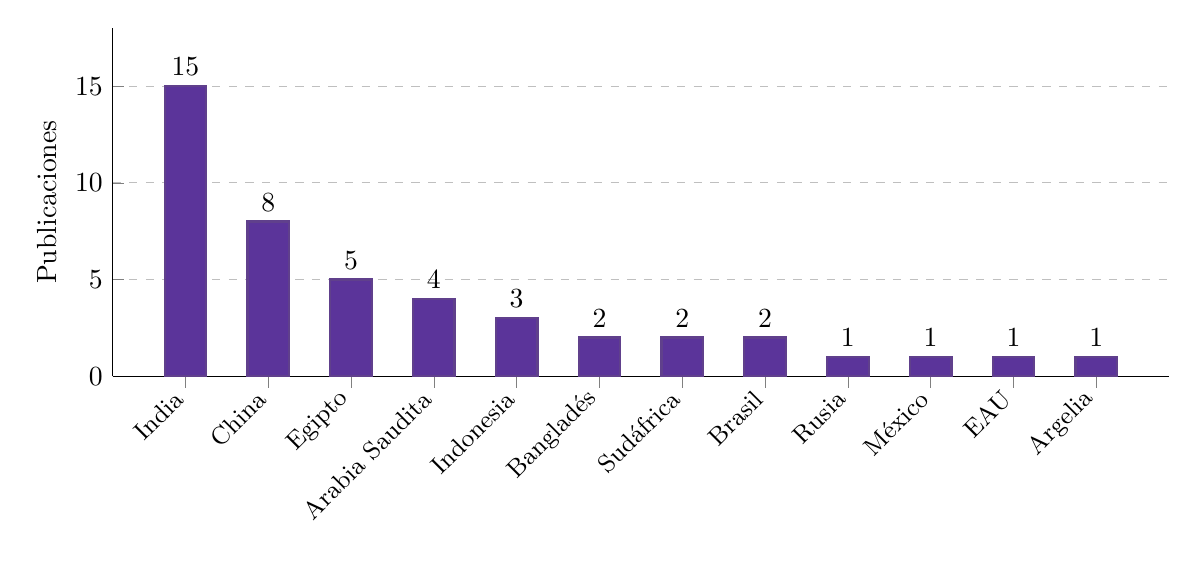
\begin{tikzpicture}
  \begin{axis}[
    ybar,
    bar width=15pt,
    width=15cm,
    height=6cm,
    ylabel={Publicaciones},
    symbolic x coords={India, China, Egipto, Arabia Saudita, Indonesia,
      Bangladés, Sudáfrica, Brasil, Rusia, México,
    EAU, Argelia},
    xtick=data,
    xticklabel style={rotate=45, anchor=east, font=\small},
    nodes near coords,
    nodes near coords align={vertical},
    ymin=0,
    ymax=18,
    enlarge x limits=0.08,
    axis lines*=left,
    ymajorgrids=true,
    grid style=dashed,
    ]

    \addplot[fill=RoyalPurple, draw=RoyalPurple!80!black, thick] coordinates {
      (India, 15)
      (China, 8)
      (Egipto, 5)
      (Arabia Saudita, 4)
      (Indonesia, 3)
      (Bangladés, 2)
      (Sudáfrica, 2)
      (Brasil, 2)
      (Rusia, 1)
      (México, 1)
      (EAU, 1)
      (Argelia, 1)
    };
  \end{axis}
\end{tikzpicture}
\end{document}
